\documentclass{article}


%%%% packages and definitions (optional)
\usepackage{graphicx} % allows inclusion of graphics
\usepackage{graphics}
\usepackage{placeins}
\usepackage{booktabs} % nice rules (thick lines) for tables
\usepackage{microtype} % improves typography for PDF


\usepackage{xcolor, colortbl}
\definecolor{Lightred}{rgb}{1.92,0.81,0.82}
\newcolumntype{a}{>{\columncolor{Lightred}}c}
\definecolor{LightCyan}{rgb}{0.88,1,1}
\newcolumntype{q}{>{\columncolor{LightCyan}}c}

\newcommand{\SN}{S$_N$}
\renewcommand{\vec}[1]{\bm{#1}} %vector is bold italic
\newcommand{\vd}{\bm{\cdot}} % slightly bold vector dot
\newcommand{\grad}{\vec{\nabla}} % gradient
\newcommand{\ud}{\mathop{}\!\mathrm{d}} % upright derivative symbol
\graphicspath{ {images/} }

\newcommand{\Cyclus}{\textsc{Cyclus}}%
\newcommand{\Cycamore}{\textsc{Cycamore}}%

% tikz %
\usepackage{tikz-cd}
\usepackage{tikz}
\usetikzlibrary{positioning, arrows, decorations, shapes}

\usetikzlibrary{shapes.geometric,arrows}
\tikzstyle{process} = [rectangle, rounded corners, minimum width=3cm, minimum height=1cm,text centered, draw=black, fill=blue!30]
\tikzstyle{object} = [ellipse, rounded corners, minimum width=3cm, minimum height=1cm,text centered, draw=black, fill=green!30]
\tikzstyle{arrow} = [thick,->,>=stealth]

%%%% Acronym support

\usepackage[acronym,toc]{glossaries}
\newacronym{NNL}{NNL}{National Nuclear Laboratory}
\newacronym{MA}{MA}{minor actinide}
\newacronym{DU}{DU}{depleted uranium}
\newacronym{LWR}{LWR}{Light Water Reactor}
\newacronym{MOX}{MOX}{Mixed Oxide Fuel}
\newacronym{SFR}{SFR}{Sodium-cooled Fast Reactor}
\newacronym{FLM}{FLM}{Fuel Loading Model}
\newacronym{EFMC}{EFMC}{effective fissile mass coefficient}
\newacronym{ORNL}{ORNL}{Oak Ridge National Laboratory}
\newacronym{PWR}{PWR}{Pressurized Water Reactor}
\newacronym{FIT}{FIT}{Functionality Isolation Test}
\newacronym{MSR}{MSR}{Molten Salt Reactor}
\newacronym{PRISM}{PRISM}{Power Reactor Innovative Small Module}
\newacronym{UNF-ST&DARDS}{UNF-ST&DARDS}{Used Nuclear Fuel-Storage, Transportation and Disposal Analysis Resource and Data System}
\newacronym{UNF-STANDARDS}{UNF-STANDARDS}{Used Nuclear Fuel-Storage, Transportation and Disposal Analysis Resource and Data System}
\newacronym{UDB}{UDB}{Unified Database}
\newacronym{UNF}{UNF}{used nuclear fuel}

\makeglossaries

%%%%%%%%%%%%%%actual words%%%%%%%%%%%%%%%%%%%%%%%%%%%%%%%%%%%%%%%%%%%%%%%%%%%%5
\begin{document}
\begin{titlepage}
    \centering
    {\scshape\LARGE \gls{UNF-STANDARDS} Sensitivity Study\par}
    \vspace{1cm}
    {\scshape\Large Effects of finer UNF composition resolution on transition scenarios \par}
    \vspace{2cm}
    {\Large\itshape Jin Whan Bae,
    Joshua L. Peterson-Droogh, Andrew Worrall \par}
    \vfill
    Oak Ridge National Laboratory, Oak Ridge, TN
    \vfill
    \vfill

% Bottom of the page
    {\large \today\par}
\end{titlepage}




\section{Introduction}
The \gls{UNF-STANDARDS} incorporates the \gls{UDB}, which is a comprehensive, controlled \gls{UNF}
system database, for nuclear analysis capabilities \cite{banerjee_unf-ST&DARDS:_2016}. The
\gls{UNF-STANDARDS} provides various nuclear safety and analyses capabilities such as:
\begin{enumerate}
    \item Depletion and decay
    \item Criticality analysis for casks
    \item Thermal analysis for casks
    \item Shielding analysis for casks
    \item Containment analysis for casks
\end{enumerate}

In this report, only the depletion and decay aspect is utilized, where we look at the effect
of having a very fine-resolution profile of the \gls{UNF} inventory compared to a lower
resolution profile of the \gls{UNF} in the context of transition scenarios.
The goal of this report is to quantitatively measure
how much error is introduced by generalizing the discharge composition of the \gls{UNF}
inventory.


\section{\gls{UNF-STANDARDS}}
The original motivation for the \gls{UNF-STANDARDS} was to provide a national resource
for the transport, storage, and disposal of \gls{UNF} in the United States. However,
the very fine resolution of the composition of the \gls{UNF} inventory (for individual
assemblies) make it an attractive resource for fuel cycle simulations. The fine
resolution of the \gls{MA} and uranium inventory in the \glspl{UNF} can allow for an
accurate assessment on the viability and the rapidity of fuel cycle transitions,
given that legacy fuel can be reprocessed.


\section{Method}
First, I acquire the depletion and decay data from the \gls{UNF-STANDARDS}, through
personal contact with Kaushik Banerjee at \gls{ORNL}. For security reasons, I was
only able to obtain the compositions of all the assemblies after one year of cooling.
Also, the reactors in the data are listed as ids, not names, for security reasons.

Then I loosely coupled the database with \Cyclus, the agent-based
fuel cycle simulation tool. \Cyclus allows for the user to develop any module using
either C++ or Python. I created a simple module (\texttt{udb\_reactor}) in python where the `reactor' would
discharge fuel according to the time, mass, and composition data from \gls{UNF-STANDARDS}.
The discharged fuel is then traded in the \Cyclus framework to be either stored,
reprocessed, or disposed.

For the average composition, I find the average burnup and enrichment and find an assembly
closest to the average values. Then I use the composition of the assembly as a recipe so that
all fuel the \texttt{udb\_reactor} outputs is in that composition. The discharge time
and the mass of the assemblies remain the same.


\section{Results}

\iffalse

\begin{figure}
        \centering
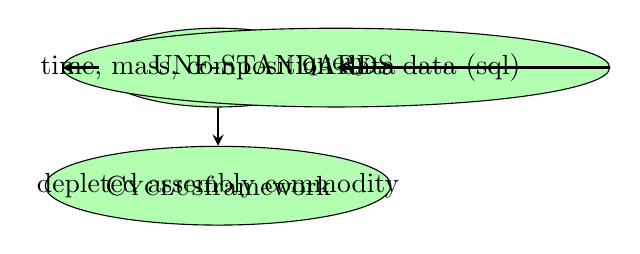
\begin{tikzpicture}[node distance=1.5cm]
\node (udbr) [object] {udb\_reactor};
\node (data) [object, right of=udbr] {\gls{UNF-STANDARDS} data (sql)};
\node (cyclus) [object, below of=udbr] {\Cyclus framework};

\draw [arrow] (udbr) -- (data)node[]{query}; 
\draw [arrow] (data) -- (udbr)node[]{time, mass, composition data}; 
\draw [arrow] (udbr) -- (cyclus)node[]{depleted assembly commodity};
\end{tikzpicture}
\caption{}
\label{diag:comp}
\end{figure}

\fi




\FloatBarrier

\section{Conclusion}

\bibliographystyle{unsrt}
\bibliography{bib}


\end{document}
